\documentclass[svgnames]{beamer}
\mode<presentation>
\usefonttheme{serif}
\usecolortheme{dove}
\useinnertheme{rounded}
%\useoutertheme{smoothbars}
\setbeamercolor{item projected}{fg=black}
\setbeamertemplate{navigation symbols}{}

\usepackage[english]{babel}
\usepackage[latin1]{inputenc}
\usepackage{times}
\usepackage{amsthm,amssymb,amsmath,graphicx}
\usepackage{color}
\usepackage{gastex}
\usepackage{framed}
\usepackage{graphicx}
\usepackage{multicol}
\usepackage{ulem}
\usepackage{ifthen}
\usepackage{tikz}

%%%%%%%%%%%%%%%%%%%%%%%%%%%%%%%%%%%%%%%%%%%%%%%%%%%%%%%%%%%%%%%%%%%%%%%%%%%%%%%%%%%%%%%%
%%%%%%%%%%%%%%%%%%%% A non-original creation by Nathanaël Fijalkow and Victor Marsault %

\setbeamertemplate{frametitle}{
  \vskip-2pt
  \begin{beamercolorbox}[rightskip=2cm,leftskip=1em,dp=1ex,wd=12.8cm]{frametitle}
    \vskip2pt
    \usebeamercolor{frametitle}
    \begin{tikzpicture}
      \useasboundingbox (0,0) rectangle (0,0); 
      \ifthenelse{\insertframenumber<\inserttotalframenumber}
      { 
        \pgfmathsetmacro{\aimangle}{90-(\insertframenumber*360/\inserttotalframenumber)}
        \fill [fill=frametitle.fg,thin, color=gray!50,draw=black] (11.8,.2) -- (11.8,.6) arc (90:\aimangle:0.4) -- cycle;

      }{ 
        \fill[fill=frametitle.fg,thin, color=gray!50,draw=black] (11.8,0.2) circle (.4);
      }
      \fill[fill=frametitle.fg,thin, color=white,draw=black] (11.8,0.2) circle (.3);
      \node at (11.8, .2) [black,circle]{\normalsize\insertframenumber};
    \end{tikzpicture}
    \insertframetitle
    \vskip2pt
  \end{beamercolorbox}
}
%%%%%%%%%%%%%%%%%%%%%%%%%%%%%%%%%%%%%%%%%%%%%%%%%%%%%%%%%%%%%%%%%%%%%%%%%%%%%%%%%%%%%%%

\setbeamertemplate{blocks}[rounded]
\setbeamercolor{block title}{bg=normal text.bg!90!black}
\setbeamercolor{block body}{bg=normal text.bg!95!black}

\renewcommand{\AA}{\mathcal{A}}

\newcommand{\PSPACE}{\mathrm{PSPACE}}
\newcommand{\BB}{\mathcal{B}}
\newcommand{\CC}{\mathcal{C}}
\newcommand{\JJ}{\mathcal{J}}
\newcommand{\DD}{\mathcal{D}}
\newcommand{\KK}{\mathcal{K}}
\newcommand{\LL}{\mathcal{L}}
\newcommand{\HH}{\mathcal{H}}
\newcommand{\GG}{\mathcal{G}}
\newcommand{\RR}{\mathbb{R}}
\newcommand{\NN}{\mathbb{N}}
\newcommand{\QQ}{\mathbb{Q}}
\newcommand{\MM}{\mathcal{M}}
\newcommand{\MMAA}{\MM_\AA}
\newcommand{\tr}[1]{\langle #1 \rangle}
\newcommand{\prob}[1]{\mathbb{P}_{#1}}
\newcommand{\stab}[1]{S(#1)}
\newcommand{\set}[1]{\{ #1 \}}
\newcommand{\val}[1]{\text{val}(#1)}
\newcommand{\merge}{\textrm{merge}}
\newcommand{\chck}{\textrm{check}}
\newcommand{\apply}{\textrm{apply}}
\newcommand{\finish}{\textrm{finish}}
\newcommand{\wait}{\textrm{wait}}
\newcommand{\delay}{\textrm{Delay}}

%\newtheorem{problem}{Open Problem}
   
\title{Algorithms for Probabilistic Automata\\
that Use Algebra}
\subtitle{S\'eminaire 68NQRT, Rennes}
\author{Nathana\"el Fijalkow}
\institute{LIAFA, Universit\'e Denis Diderot - Paris 7, France\\
Institute of Informatics, Warsaw University, Poland\\
\textbf{nath@liafa.univ-paris-diderot.fr}}

\date{January 24th, 2013}

\AtBeginSection[]
{
\addtocounter{framenumber}{-1}
  \begin{frame}<beamer>{Outline}
    \tableofcontents[currentsection]
  \end{frame}
}

\begin{document}

\addtocounter{framenumber}{-1}

\begin{frame}
  \titlepage
\end{frame}

\begin{frame}{Previously on 68NQRT: Youssouf Oualhadj}
\begin{center}
\begin{figure}
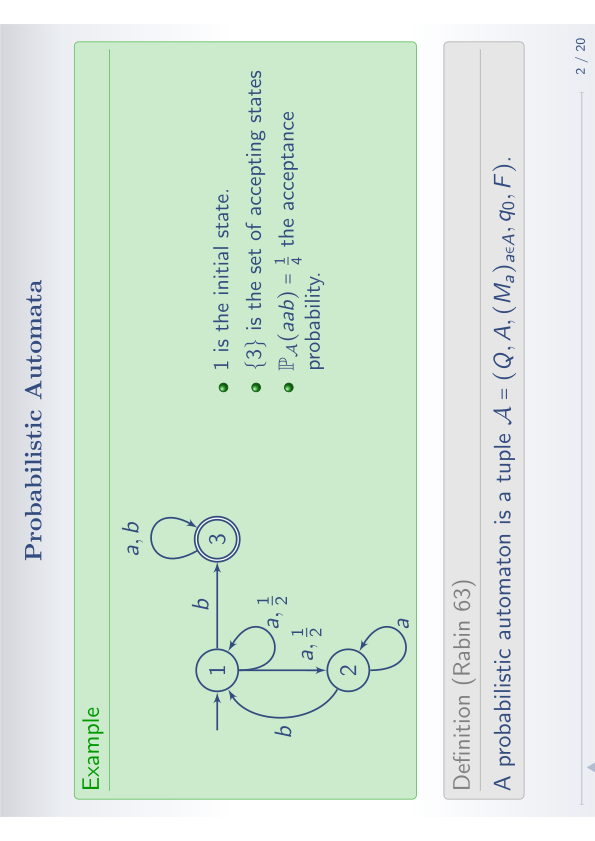
\includegraphics[scale=.9]{output}
\end{figure}
\end{center}
\end{frame}

\begin{frame}{Probabilistic automata (Rabin, 1963)}
\begin{figure}
\begin{center}
\begin{picture}(20,40)(0,-10)
	\gasset{Nw=6,Nh=6}

  	\node[Nmarks=i,iangle=0](L1)(15,15){$1$}
  	\node(L2)(0,30){$2$}
  	\node[Nmarks=r](L3)(0,0){$3$}

  	\drawedge(L1,L2){$b$}
  	\drawedge[curvedepth=-5,ELside=r](L1,L3){$a,0.4$}
  	\drawedge[curvedepth=-5,ELside=r](L3,L1){$b$}
	\drawloop(L1){$a,0.6$}
	\drawloop[loopangle=135](L2){$a,b$}
	\drawloop[loopangle=215](L3){$a$}
\end{picture}
\end{center}
\end{figure}
$$\prob{\AA} : A^* \rightarrow [0,1]$$
$$\prob{\AA}(w) \textrm{ is the probability that a run for } w \textrm{ ends up in } F$$
\end{frame}

\begin{frame}{Decision problems}
The equivalence problem:
\begin{framed}
INPUT: $\AA,\BB$ two probabilistic automata\\
OUTPUT: for all words $w \in A^*$, we have $\prob{\AA}(w) = \prob{\BB}(w)$.
\end{framed}

The emptiness problem:
\begin{framed}
INPUT: $\AA$ a probabilistic automaton and a threshold $\lambda \in \QQ$\\
OUTPUT: there exists a word $w \in A^*$ such that $\prob{\AA}(w) \ge \lambda$.
\end{framed}

The isolation problem:
\begin{framed}
INPUT: $\AA$ a probabilistic automaton and a threshold $\lambda \in \QQ$\\
OUTPUT: there exists $\varepsilon > 0$ such that
for all words $w \in A^*$, we have $\prob{\AA}(w) \notin [\lambda - \varepsilon ; \lambda + \varepsilon]$.
\end{framed}
\end{frame}

\begin{frame}{This talk}

\begin{center}
This talk is about algorithms based on \textit{algebra}.
\end{center}

\end{frame}

\begin{frame}{Weighted automata using algebra (Sch\"utzenberger)}
\vspace*{1em}
\begin{figure}
\begin{center}
\begin{picture}(60,14)(0,0)
	\gasset{Nw=6,Nh=6,loopdiam=6}

  	\node[Nmarks=i,iangle=-90](0)(20,5){$0$}
  	\node(1)(40,5){$1$}
  	\node[Nmarks=r](F)(60,5){$F$}
  	\node(bottom)(0,5){$\perp$}

	\drawloop(0){$a,0.3$}
	\drawloop(1){$a$}
	\drawloop[loopangle=0](F){$a,b$}
	\drawloop[loopangle=180](bottom){$a,b$}

  	\drawedge(0,bottom){$b$}
  	\drawedge[curvedepth=2](0,1){$a,0.7$}
  	\drawedge[curvedepth=2](1,0){$b,0.5$}
  	\drawedge(1,F){$b,0.5$}
\end{picture}
\end{center}
\end{figure}
\vspace*{1.5em}

$$\tr{a} = 
\left(\begin{array}{cccc}
1 & 0 & 0 & 0 \\
0 & 0.3 & 0.7 & 0 \\
0 & 0 & 1 & 0 \\
0 & 0 & 0 & 1
\end{array}\right)
\qquad
\tr{b} = 
\left(\begin{array}{cccc}
1 & 0 & 0 & 0 \\
1 & 0 & 0 & 0 \\
0 & 0.5 & 0.5 & 0 \\
0 & 0 & 0 & 1
\end{array}\right)$$

\vspace*{1.5em}

\only<1>{
$$I = \left(\begin{array}{cccc} 0 & 1 & 0 & 0 \end{array}\right)
\qquad
F = \left(\begin{array}{c} 0 \\ 0 \\ 0 \\ 1 \end{array}\right)$$}

\only<2>{
$$\prob{\AA}(aaabaa) = I \cdot \tr{aaabaa} \cdot F = 
I \cdot \tr{a} \cdot \tr{a} \cdot \tr{a} \cdot \tr{b} \cdot \tr{a} \cdot \tr{a} \cdot F$$
}
\vspace*{10em}
\end{frame}

\section{The equivalence problem}

\begin{frame}{Decidability}
\begin{framed}
INPUT: $\AA,\BB$ two probabilistic automata\\
OUTPUT: for all words $w \in A^*$, we have $\prob{\AA}(w) = \prob{\BB}(w)$.
\end{framed}

\begin{theorem}
The equivalence problem is decidable in polynomial time.
\end{theorem}

\pause
\begin{itemize}
	\item Sch\"utzenberger (1961) -- minimization of weighted automata
	\item Tzeng (1992) -- backward algorithm
	\item Doyen, Henzinger and Raskin (2008) -- algebraic forward algorithm
	\item Kiefer, Murawski, Ouaknine, Wachter and Worrell (2010) -- randomized \textrm{NC}
\end{itemize}
\end{frame}

\begin{frame}{A simple algebraic algorithm}
A probabilistic distribution is $\delta : Q \rightarrow [0,1]$
which sums up to $1$.
\vskip2em

\begin{definition}[Bisimilarity over distributions]
Two probabilistic distributions $\delta_1$ and $\delta_2$ are bisimilar if for all words $w \in A^*$,
we have 
$$\prob{\AA}^{\delta_1}(w) = \prob{\AA}^{\delta_2}(w)\ .$$
\end{definition}

\pause
\vskip2em
The equivalence problem reduces to the bisimilarity problem of two probabilistic distributions.
\end{frame}

\begin{frame}{Checking bisimilarity}
Two probabilistic distributions $\delta_1$ and $\delta_2$ are bisimilar if for all words $w \in A^*$,
we have 
$$\prob{\AA}^{\delta_1}(w) = \prob{\AA}^{\delta_2}(w)\ .$$


$$\textrm{Equivalently:} \qquad \left\{
\begin{array}{c}
\prob{\AA}^{\delta_1}(\varepsilon) = \prob{\AA}^{\delta_2}(\varepsilon) \\[1ex]
\prob{\AA}^{\delta_1}(a) = \prob{\AA}^{\delta_2}(a) \\[1ex]
\prob{\AA}^{\delta_1}(b) = \prob{\AA}^{\delta_2}(b) \\[1ex]
\prob{\AA}^{\delta_1}(aa) = \prob{\AA}^{\delta_2}(aa) \\[1ex]
\ldots
\end{array}
\right.$$

\pause
Let $N = |Q|$.
\begin{itemize}
	\item each line is a linear equation involving $N$ variables;
	\item there are at most $N$ independent linear equations;
	\item no independent equations are added for words of length $\ge N$.
\end{itemize}
\end{frame}

\begin{frame}{Linear algebra and dimensions}

Denote $X$ and $Y$ the vectors for $\delta_1$ and $\delta_2$.
$$\left\{
\begin{array}{c}
{}^t (X-Y) \cdot F = 0 \\[1ex]
{}^t (X-Y) \cdot \tr{a} \cdot F = 0 \\[1ex]
{}^t (X-Y) \cdot \tr{b} \cdot F = 0 \\[1ex]
{}^t (X-Y) \cdot \tr{aa} \cdot F = 0 \\[1ex]
\ldots
\end{array}
\right.$$

\pause
Denote $W_k = \langle \set{ \tr{w} \cdot F \mid w \in A^{\le k} } \rangle$, generated vector space in $\RR^N$.

The solutions live in $W_k^{\bot}$, orthogonal subspace of $W_k$.

\pause
$$W_0 \subseteq W_1 \subseteq W_2 \subseteq \ldots \ .$$

\begin{itemize}
	\item For all $k$, if $W_k = W_{k+1}$, then $W_{k+1} = W_{k+2}$;
	\item Reasoning on dimensions shows that the sequence stabilizes before $N$ steps.
\end{itemize}
\end{frame}

\begin{frame}{Conclusion for the equivalence problem}
\begin{center}
With basic algebraic arguments we get a very simple algorithm
checking the equivalence of two probabilistic automata,\\
which runs in cubic time.
\vskip2em
Bottom line: $(\RR,+,\times)$ is a field,\\
hence linear algebra comes into play!
\end{center}
\end{frame}

\section{The isolation problem}

\begin{frame}{Undecidability}
\begin{framed}
INPUT: $\AA$ a probabilistic automaton and a threshold $\lambda \in \QQ$\\
OUTPUT: there exists $\varepsilon > 0$ such that
for all words $w \in A^*$, we have $\prob{\AA}(w) \notin [\lambda - \varepsilon ; \lambda + \varepsilon]$.
\end{framed}

\begin{theorem}[Bertoni, 1974]
The isolation problem is undecidable for $0 < \lambda < 1$.
\end{theorem}

\pause
What about $\lambda = 1$ and $\lambda = 0$?
\end{frame}

\begin{frame}{A special case: the value $1$ problem}

For $\lambda = 1$ the isolation problem can be formulated as:
\begin{center}
``are there words accepted with probability arbitrarily close to $1$''.
\end{center}
\pause
\vskip1em
Equivalently, define $\val{\AA} = \sup_w \prob{\AA}(w)$,
then the problem is:
\begin{center}
``$\val{\AA} \stackrel{?}{=} 1$''.
\end{center}

\pause
\begin{theorem}[Gimbert and Oualhadj, 2010]
The value $1$ problem is undecidable.
\end{theorem}
\end{frame}

\begin{frame}{An intuition}

\begin{figure}
\begin{center}
\begin{picture}(60,35)(0,0)
	\gasset{Nw=7,Nh=7}

  	\node[Nmarks=i,iangle=-90](0)(30,15){$0$}
  	\node(L1)(0,10){$L_1$}
  	\node[Nmarks=r](L2)(0,30){$L_2$}
  	\node(R1)(60,10){$R_1$}
  	\node(R2)(60,30){$R_2$}

	\drawloop(0){$a$}

  	\drawedge[curvedepth=5,ELside=l](0,L1){$b,\frac{1}{2}$}
  	\drawedge[curvedepth=5,ELside=l](L1,0){$a,1-x$}
  	\drawedge(L1,L2){$b$}
	\drawloop[loopangle=-135](L1){$a,x$}
	\drawloop[loopangle=90](L2){$a,b$}

  	\drawedge[curvedepth=-5,ELside=r](0,R1){$b,\frac{1}{2}$}
  	\drawedge[curvedepth=-5,ELside=r](R1,0){$a,x$}
  	\drawedge[ELside=r](R1,R2){$b$}
	\drawloop[loopangle=-45](R1){$a,1-x$}
	\drawloop(R2){$a,b$}
\end{picture}
\end{center}
\end{figure}
\begin{center}
has value $1$ if and only if $x > \frac{1}{2}$.
\end{center}
\end{frame}

\begin{frame}{A very restricted case}
\begin{theorem}[F., Gimbert and Oualhadj, 2011]
The isolation problem is (still) undecidable if we randomise only on \textbf{one} transition.
\end{theorem}
\end{frame}

\begin{frame}{Objective}
Define a \textit{partial} algorithm to decide the value $1$ problem,
by \textbf{algebraic} and \textbf{non-numerical} means.
\pause

\begin{itemize}
	\item \textbf{algebraic:} focus on the automaton structure,
	\item \textbf{non-numerical:} abstract away the values.
\end{itemize}

\pause
Hence we consider non-deterministic automata:
we project $(\RR,+,\cdot)$ into the boolean semiring $(\set{0,1},+,\cdot)$.
\pause
\begin{figure}
\begin{center}
\begin{picture}(20,15)(0,5)
	\gasset{Nw=6,Nh=6}

  	\node[Nmarks=i,iangle=180](1)(0,5){$1$}
  	\node[Nmarks=r](2)(20,5){$2$}

	\drawloop(1){$a$}
  	\drawedge(1,2){$a$}
	\drawloop(2){$a$}
\end{picture}
\end{center}
\end{figure}
\end{frame}

\begin{frame}{An example}
\begin{figure}
\begin{center}
\begin{picture}(60,15)(0,-5)
	\gasset{Nw=6,Nh=6,loopdiam=6}

  	\node[Nmarks=i,iangle=-90](0)(20,5){$0$}
  	\node(1)(40,5){$1$}
  	\node[Nmarks=r](F)(60,5){$F$}
  	\node(bottom)(0,5){$\perp$}

	\drawloop(0){$a$}
	\drawloop(1){$a$}
	\drawloop[loopangle=0](F){$a,b$}
	\drawloop[loopangle=180](bottom){$a,b$}

  	\drawedge(0,bottom){$b$}
  	\drawedge[curvedepth=2](0,1){$a$}
  	\drawedge[curvedepth=2](1,0){$b$}
  	\drawedge(1,F){$b$}
\end{picture}
\invisible<1,5,6>{
\begin{picture}(60,10)(0,0)
	\gasset{Nw=5,Nh=5,loopdiam=4}

	\put(-20,4){$\tr{a}$}

  	\node(0)(20,5){$0$}
  	\node(1)(40,5){$1$}
  	\node[Nmarks=r](F)(60,5){$F$}
  	\node(bottom)(0,5){$\perp$}

	\drawloop(0){}
	\drawloop(1){}
	\drawloop[loopangle=0](F){}
	\drawloop[loopangle=180](bottom){}

  	\drawedge(0,1){}
\end{picture}}
\invisible<1,2,4,6>{
\begin{picture}(60,10)(0,0)
	\gasset{Nw=5,Nh=5,loopdiam=4}

	\put(-20,4){$\tr{b}$}

  	\node(0)(20,5){$0$}
  	\node(1)(40,5){$1$}
  	\node[Nmarks=r](F)(60,5){$F$}
  	\node(bottom)(0,5){$\perp$}

	\drawloop[loopangle=0](F){}
	\drawloop[loopangle=180](bottom){}

  	\drawedge(0,bottom){}
  	\drawedge(1,0){}
  	\drawedge(1,F){}
\end{picture}}
\invisible<1,2,3,6>{
\begin{picture}(60,10)(0,0)
	\gasset{Nw=5,Nh=5,loopdiam=4}

	\put(-20,4){$\tr{a^\sharp}$}

  	\node(0)(20,5){$0$}
  	\node(1)(40,5){$1$}
  	\node[Nmarks=r](F)(60,5){$F$}
  	\node(bottom)(0,5){$\perp$}

	\drawloop(1){}
	\drawloop[loopangle=0](F){}
	\drawloop[loopangle=180](bottom){}

  	\drawedge(0,1){}
\end{picture}}
\invisible<1,2,3,4>{
\begin{picture}(60,10)(0,0)
	\gasset{Nw=5,Nh=5,loopdiam=4}

	\put(-22,4){$\tr{a^\sharp \cdot b}$}

  	\node(0)(20,5){$0$}
  	\node(1)(40,5){$1$}
  	\node[Nmarks=r](F)(60,5){$F$}
  	\node(bottom)(0,5){$\perp$}

	\drawloop(0){}
	\drawloop[loopangle=0](F){}
	\drawloop[loopangle=180](bottom){}

  	\drawedge[curvedepth=-4](0,F){}
  	\drawedge(1,0){}
  	\drawedge(1,F){}
\end{picture}}
\invisible<1,2,3,4,5>{
\begin{picture}(60,10)(0,0)
	\gasset{Nw=5,Nh=5,loopdiam=4}

	\put(-25,4){$\tr{(a^\sharp \cdot b)^\sharp}$}

  	\node(0)(20,5){$0$}
  	\node(1)(40,5){$1$}
  	\node[Nmarks=r](F)(60,5){$F$}
  	\node(bottom)(0,5){$\perp$}

	\drawloop[loopangle=0](F){}
	\drawloop[loopangle=180](bottom){}

  	\drawedge[curvedepth=-4](0,F){}
  	\drawedge(1,F){}
\end{picture}}
\end{center}
\end{figure}
\pause\pause\pause\pause\pause\pause
\end{frame}

\begin{frame}{Stabilization monoids (Colcombet)}
This is an algebraic structure with two operations:
\begin{itemize}
	\item binary composition
	\item stabilization, denoted $\sharp$.
\end{itemize}
\end{frame}

\begin{frame}{Boolean matrices representations}
\vspace*{1em}
\begin{figure}
\begin{center}
\begin{picture}(60,14)(0,0)
	\gasset{Nw=6,Nh=6,loopdiam=6}

  	\node[Nmarks=i,iangle=-90](0)(20,5){$0$}
  	\node(1)(40,5){$1$}
  	\node[Nmarks=r](F)(60,5){$F$}
  	\node(bottom)(0,5){$\perp$}

	\drawloop(0){$a$}
	\drawloop(1){$a$}
	\drawloop[loopangle=0](F){$a,b$}
	\drawloop[loopangle=180](bottom){$a,b$}

  	\drawedge(0,bottom){$b$}
  	\drawedge[curvedepth=2](0,1){$a$}
  	\drawedge[curvedepth=2](1,0){$b$}
  	\drawedge(1,F){$b$}
\end{picture}
\end{center}
\end{figure}
\vspace*{1em}

$$\tr{a} = 
\left(\begin{array}{cccc}
1 & 0 & 0 & 0 \\
0 & 1 & 1 & 0 \\
0 & 0 & 1 & 0 \\
0 & 0 & 0 & 1
\end{array}\right)
\qquad
\tr{b} = 
\left(\begin{array}{cccc}
1 & 0 & 0 & 0 \\
1 & 0 & 0 & 0 \\
0 & 1 & 1 & 0 \\
0 & 0 & 0 & 1
\end{array}\right)$$

\vspace*{1em}

$$I \cdot \tr{u} \cdot F = 1 \quad \textrm{ if and only if } \quad \prob{\AA}(u) > 0$$
\end{frame}

\begin{frame}{Defining stabilization}
\vspace*{3em}
\begin{figure}
\begin{center}
\begin{picture}(20,10)(0,0)
	\gasset{Nw=6,Nh=6}

  	\node[Nmarks=i,iangle=180](1)(0,5){$1$}
  	\node[Nmarks=r](2)(20,5){$2$}

	\drawloop(1){$a$}
  	\drawedge(1,2){$a$}
	\drawloop(2){$a$}
\end{picture}
\end{center}
\end{figure}
\vspace*{1.5em}
$$\only<1,2,3>{
\tr{a} = 
\left(\begin{array}{ccc}
1 & 1 \\
0 & 1
\end{array}\right)
	}
\qquad
\only<2,3>{
\tr{a^\sharp} = 
\left(\begin{array}{ccc}
0 & 1\\
0 & 1
\end{array}\right)}$$
\vspace*{1em}
In $\tr{a}$, the state $1$ is transient and the state $2$ is recurrent.

\vspace*{1em}
$$\only<3>{M^\sharp(s,t) = 
\left\{\begin{array}{ll}
1 & \textrm{if } M(s,t) = 1 \textrm{ and } t \textrm{ recurrent in } M,\\
0 & \textrm{otherwise.}
\end{array}\right.}$$
\vspace*{10em}
\end{frame}


\begin{frame}{The algorithm}
Compute a monoid inside the \textbf{finite} monoid $\MM_{Q \times Q}(\set{0,1},+,\times)$.

\begin{itemize}
	\item Compute $\tr{a}$ for $a \in A$:
$$\tr{a}(s,t) = 
\left\{\begin{array}{ll}
1 & \textrm{if } \prob{\AA}(s \xrightarrow{a} t) > 0,\\
0 & \textrm{otherwise.}
\end{array}\right.$$	
	\item Close under product and stabilization.
	\item \pause If there exists a matrix $M$ such that 
	$$\forall t \in Q, \quad M(s_0,t) = 1 \Rightarrow t \in F$$
	then ``$\AA$ has value $1$'',
	otherwise ``$\AA$ does not have value $1$''.
\end{itemize}
\end{frame}

\begin{frame}{Correctness}
\begin{theorem}
If there exists a matrix $M$ such that 
$$\forall t \in Q, \quad M(s_0,t) = 1 \Rightarrow t \in F$$
then $\AA$ has value $1$.
\end{theorem}
\pause
But the value $1$ problem is undecidable, so\ldots
\end{frame}

\begin{frame}{No completeness}
\begin{figure}
\begin{center}
\begin{picture}(60,35)(0,0)
	\gasset{Nw=7,Nh=7}

  	\node[Nmarks=i,iangle=-90](0)(30,15){$0$}
  	\node(L1)(0,10){$L_1$}
  	\node[Nmarks=r](L2)(0,30){$L_2$}
  	\node(R1)(60,10){$R_1$}
  	\node(R2)(60,30){$R_2$}

	\drawloop(0){$a$}

  	\drawedge[curvedepth=5,ELside=l](0,L1){$b,\frac{1}{2}$}
  	\drawedge[curvedepth=5,ELside=l](L1,0){$a,1-x$}
  	\drawedge(L1,L2){$b$}
	\drawloop[loopangle=-135](L1){$a,x$}
	\drawloop[loopangle=90](L2){$a,b$}

  	\drawedge[curvedepth=-5,ELside=r](0,R1){$b,\frac{1}{2}$}
  	\drawedge[curvedepth=-5,ELside=r](R1,0){$a,x$}
  	\drawedge[ELside=r](R1,R2){$b$}
	\drawloop[loopangle=-45](R1){$a,1-x$}
	\drawloop(R2){$a,b$}
\end{picture}
\end{center}
\end{figure}

%For all matrices $M$,
%$$\exists t \in Q, \quad M(s_0,t) = 1 \wedge t \notin F$$
%but $\AA$ has value $1$. 

Left and right parts are symmetric, so for all $M$:
$$M(0,L_2) = 1 \Longleftrightarrow M(0,R_2) = 1.$$
\end{frame}

\begin{frame}{A leak}
\begin{figure}
\begin{center}
\begin{picture}(50,30)(0,0)
	\gasset{Nw=6,Nh=6}

  	\node[Nmarks=i,iangle=0](L1)(15,15){$1$}
  	\node(L2)(0,30){$2$}
  	\node[Nmarks=r](L3)(0,0){$3$}

  	\drawedge(L1,L2){$b$}
  	\drawedge[curvedepth=-5,ELside=r](L1,L3){$a$}
  	\drawedge[curvedepth=-5,ELside=r](L3,L1){$b$}
	\drawloop(L1){$a$}
	\drawloop[loopangle=135](L2){$a,b$}
	\drawloop[loopangle=215](L3){$a$}

	\drawline[linewidth=.3,AHnb=0](26,-3)(26,40)

\pause

	\put(45,-10){$\tr{a^\sharp \cdot b}$}

  	\node(L1b)(55,15){$1$}
  	\node(L2b)(40,30){$2$}
  	\node[Nmarks=r](L3b)(40,0){$3$}

  	\drawedge(L3b,L1b){}
	\drawloop(L1b){}
	\drawloop[loopangle=135](L2b){}

\only<3>{\drawedge[dash={1}0](L1b,L2b){$\varepsilon$}}
\end{picture}
\end{center}
\end{figure}
\pause
\vskip2em
\begin{center}
There is a leak from $1$ to $2$.
\end{center}
\pause
\begin{definition}
An automaton $\AA$ is leaktight if it has no leak.
\end{definition}
\end{frame}

\begin{frame}{Leaktight automata}

\begin{theorem}[F.,Gimbert and Oualhadj, LICS 2012]
The algorithm is complete for leaktight automata.

Hence, the value $1$ problem is decidable for leaktight automata.
\end{theorem}

\vskip2em
The proof relies on Simon's factorization forest theorem.
\end{frame}

\section{The emptiness problem}

\begin{frame}{Undecidability}

\begin{framed}
INPUT: $\AA$ a probabilistic automaton and a threshold $\lambda \in \QQ$\\
OUTPUT: there exists a word $w \in A^*$ such that $\prob{\AA}(w) \ge \lambda$.
\end{framed}

\begin{theorem}[Paz, 1971]
The emptiness problem is undecidable for $0 < \lambda < 1$.
\end{theorem}
\end{frame}

\begin{frame}{Approximations}
\begin{framed}
INPUT: $\AA$ a probabilistic automaton and a threshold $\lambda \in \QQ$\\
OUTPUT: 
\begin{itemize}
	\item if there exists a word $w \in A^*$ such that $\prob{\AA}(w) \ge \lambda$: YES,
	\item if for all words $w$ we have $\prob{\AA}(w) < \lambda$: NO.
\end{itemize}
\end{framed}

Approximated:
\begin{framed}
INPUT: $\AA$ a probabilistic automaton, two thresholds $\lambda,\varepsilon \in \QQ$\\
OUTPUT: 
\begin{itemize}
	\item if there exists a word $w \in A^*$ such that $\prob{\AA}(w) \ge \lambda$: YES,
	\item if for all words $w$ we have $\prob{\AA}(w) \le \lambda - \varepsilon$: NO.
\end{itemize}
\end{framed}
\end{frame}

\begin{frame}{Inapproximability}
\begin{framed}
INPUT: $\AA$ a probabilistic automaton, two thresholds $\lambda,\varepsilon \in \QQ$\\
OUTPUT: 
\begin{itemize}
	\item if there exists a word $w \in A^*$ such that $\prob{\AA}(w) \ge \lambda$: YES,
	\item if for all words $w$ we have $\prob{\AA}(w) \le \lambda - \varepsilon$: NO.
\end{itemize}
\end{framed}

\pause

\begin{theorem}[Condon and Lipton, 1989]
There is no approximation algorithm for the emptiness problem.
\end{theorem}
\end{frame}

\begin{frame}{Unary automata (\textit{a.k.a} Markov chains)}

Markov chains are the subcase where the alphabet has only one letter.

\begin{theorem}[Daviaud and F.]
There is an approximation algorithm for Markov chains.
\end{theorem}
%\end{frame}
%
%\begin{frame}{An approximation algorithm for unary automata}
%The alphabet is $A = \set{a}$,
%we want to determine whether there exists an integer $n$ such that 
%$\prob{\AA}(a^n) \ge \lambda$.
%
%\vskip2em
%We reduce the problem to finitely many instances of the subproblem where:
%\begin{enumerate}
%	\item all states are recurrent;
%	\item all states are aperiodic.
%\end{enumerate}
%\end{frame}
%
%\begin{frame}{Restricting to recurrent states}
%\begin{figure}
%\begin{center}
%\begin{picture}(20,10)(0,0)
%	\gasset{Nw=6,Nh=6}
%
%  	\node[Nmarks=i,iangle=180](1)(0,5){$1$}
%  	\node[Nmarks=r](2)(20,5){$2$}
%
%	\drawloop(1){$.3$}
%  	\drawedge(1,2){$.7$}
%	\drawloop(2){$1$}
%\end{picture}
%\end{center}
%\end{figure}
%\vspace*{1em}
%The state $1$ is transient and the state $2$ is recurrent.
%
%\pause
%\vskip2em
%\textit{Rough idea}: for ``long'' words, the probability to be in transient states is negligible,
%so can be approximated by $0$.
%\end{frame}
%
%\begin{frame}{Restricting to aperiodic states}
%\begin{figure}
%\begin{center}
%\begin{picture}(20,10)(0,0)
%	\gasset{Nw=6,Nh=6}
%
%  	\node[Nmarks=i,iangle=-90](1)(0,5){$1$}
%  	\node(2)(20,5){$2$}
%
%  	\drawedge[curvedepth=5](1,2){}
%  	\drawedge[curvedepth=5](2,1){}
%\end{picture}
%\end{center}
%\end{figure}
%The states $1$ and $2$ are periodic, with a period $2$.
%\pause
%\vskip2em
%\textit{Rough idea}: we consider two automata, each reading two letters at a time.
%\begin{figure}
%\begin{center}
%\begin{picture}(20,10)(0,0)
%	\gasset{Nw=6,Nh=6}
%
%  	\node[Nmarks=i,iangle=-90](1)(0,5){$1$}
%  	\node(2)(20,5){$2$}
%
%  	\drawloop[loopangle=180](1){}
%  	\drawloop[loopangle=0](2){}
%\end{picture}
%\end{center}
%\end{figure}
%\end{frame}
%
%\begin{frame}{A simple algorithm for the subproblem}
%
%Denote by $M$ the transition matrix for the unique letter: $M = \tr{a}$.
%
%\begin{lemma}[monotonicity]
%If all states are recurrent and aperiodic, then 
%\begin{itemize}
%	\item the sequence $(M^n)_{n \in \NN}$ converges to $M_\infty$;
%	\item the sequence $(||M^n - M_\infty||_1)_{n \in \NN}$ is non-increasing (and converges to $0$).
%\end{itemize}
%\end{lemma}
%
%\pause
%\vskip1em
%Relying on this lemma, an algorithm for non-emptiness is:
%\begin{itemize}
%	\item compute all acceptance probabilities until $|| M^n - M_\infty ||_1 < \varepsilon$;
%	\item compute the acceptance probability in the limit, \textit{i.e} for $M_\infty$.
%\end{itemize}
%\end{frame}
%
%\begin{frame}{Conclusion for the emptiness problem}
%
%The emptiness problem is in general undecidable and even not approximable.
%\vskip1em
%However, when restricted to unary automata the emptiness problem is approximable.
\vskip1em
\begin{problem}
Is the emptiness problem decidable for Markov chains?
\end{problem}

\pause
\end{frame}

\begin{frame}{Conclusions}
A good understanding of algebra often allows to design simple algorithms
for probabilistic automata.
\begin{framed}
The \textit{equivalence problem} is decidable in polynomial time with a simple algebraic algorithm.
\end{framed}

\begin{framed}
The \textit{isolation problem} is undecidable,
but there exists a partial algebraic algorithm.
\end{framed}

\begin{framed}
The \textit{emptiness problem} is undecidable and in general not even approximable.

Is it decidable for Markov chains?
\end{framed}
\end{frame}

\begin{frame}{The end.}
Thanks for your attention!
\end{frame}


\end{document}